\documentclass[11pt]{article}
\usepackage{enumerate}
\usepackage{fullpage}
\usepackage{fancyhdr}
\usepackage{amsmath, amsfonts, amsthm, amssymb}
\usepackage{color}
\usepackage{mathrsfs}
\usepackage{bbm}
\setlength{\parindent}{0pt}
\setlength{\parskip}{5pt plus 1pt}
\usepackage {tikz}
\usetikzlibrary{positioning}
\definecolor{processblue}{cmyk}{0.96,0,0,0}

% for graphs
\usepackage {tikz}
\usetikzlibrary{positioning}
\definecolor{processblue}{cmyk}{0.96,0,0,0}


%%%%%%%%%%%%%%%%%%%%%%%HEADER%%%%%%%%%%%%%%%%%%%%%%%%%%%%%%
\newcommand{\myname}{Shashank Singh\footnote{sss1@andrew.cmu.edu}}
\newcommand{\myclass}{10/36-702 Statistical Machine Learning}
\newcommand{\myhwnum}{4}
\newcommand{\duedate}{Friday, April 10, 2015}
%%%%%%%%%%%%%%%%%%%%%%%%%%%%%%%%%%%%%%%%%%%%%%%%%%%%%%%%%%%

%%%%%%%%%%%%%%%%%%%%CONTENT MACROS%%%%%%%%%%%%%%%%%%%%%%%%%
\renewcommand{\qed}{\quad \ensuremath{\blacksquare}}
\newcommand{\inv}{^{-1}}
\newcommand{\dist}{\operatorname{dist}}
\newcommand{\area}{\operatorname{area}}
\newcommand{\vspan}{\operatorname{span}}
\newcommand{\Gr}{\operatorname{Gr}} % graph of a function
\renewcommand{\sp}{\operatorname{span}} % span of a set
\newcommand{\sminus}{\backslash}
\newcommand{\E}{\mathbb{E}} % expected value
\newcommand{\F}{\mathcal{F}}
\newcommand{\Fc}{\mathscr{F}} % function class
\newcommand{\pr}{\mathbb{P}} % probability
\newcommand{\Var}{\mathbb{V}} % variance
\newcommand{\Cov}{\operatorname{Cov}} % covariance
\newcommand{\N}{\mathbb{N}} % natural numbers
\newcommand{\Z}{\mathbb{Z}} % integers
\newcommand{\Q}{\mathbb{Q}} % rational numbers
\newcommand{\R}{\mathbb{R}} % real numbers
\newcommand{\A}{\mathcal{A}}
\newcommand{\B}{\mathscr{B}}
\newcommand{\X}{\mathcal{X}}
\newcommand{\C}{\mathscr{C}} % compact functions
\newcommand{\K}{\mathbb{K}} % underlying field of a linear space
\newcommand{\Ran}{\mathcal{R}} % range of a linear operator
\newcommand{\Nul}{\mathcal{N}} % null-space of a linear operator
\renewcommand{\L}{\mathcal{L}} % bounded linear functions
\newcommand{\pow}[1]{\mathcal{P}\left(#1\right)} % power set of #1
\newcommand{\e}{\varepsilon} % \varepsilon
\newcommand{\wto}{\rightharpoonup} % weak convergence
\newcommand{\wsto}{\stackrel{*}{\rightharpoonup}} % weak-* convergence
\renewcommand{\P}{\mathbb{P}}   % probability
\newcommand{\ol}{\overline}
\newcommand{\MSE}{\operatorname{MSE}} % mean squared error
\newcommand{\tr}{\operatorname{tr}} % trace operator
\renewcommand{\H}{\mathscr{H}} % Hilbert space (RKHS)
\renewcommand{\hat}{\widehat}
\newcommand{\argmin}{\operatornamewithlimits{argmin}}
\newcommand{\argmax}{\operatornamewithlimits{argmax}}
\newcommand\ind{\protect\mathpalette{\protect\independenT}{\perp}}
\def\independenT#1#2{\mathrel{\rlap{$#1#2$}\mkern2mu{#1#2}}}
%%%%%%%%%%%%%%%%%%%%%%%%%%%%%%%%%%%%%%%%%%%%%%%%%%%%%%%%%%%

\begin{document}

{\Large Homework \myhwnum} \\
Name: \myname \\
\myclass \\
Due: \duedate

\begin{enumerate}
\item
\begin{enumerate}
\item Suppose $\theta \in \R^n$. Since, $f(y; \theta)$ is a density function on
$D$ in $y$, $1 = \int_D f(y; \theta) \, dy$. Solving for $b(\theta)$ gives
$b(\theta) = \log \left( \int_D f_0(y) e^{y^T \theta} \, dy \right)$. Since
$f_0$ is a density function on $D$, it is strictly positive on a region of
positive measure. Since $e^{y^T \theta} > 0$ for all $y \in D$,
$\int_D f_0(y) e^{y^T \theta} \, dy > 0$, and so $b(\theta) < \infty$. Thus, $C
= \R^n$, which is trivially convex. \qed

\item Since the function $x \mapsto e^{y^T x}$ on $\R$ is the composition of a
convex function (exponentiation) with an affine transformation, it is convex.
Since the function $x \mapsto \int_D f_0(y) x_y \, dy$ on $D^\R$ is a convex
combination and $\log$ is concave and nondecreasing, the function
$\theta \mapsto \log \int_D f_0(y) e^{y^T \theta} \, dy$ is convex. \qed

\item Let $X$ be the matrix whose $i^{th}$ row is $x_i^T$. Then, $B$ is the
preimage of the convex set $C$ under the linear function $c \mapsto Xc$, and
so $B$ is convex. \qed

\item For any $\beta \in B$,
\[\ell(\beta; Y)
    = \log \left( \prod_{i = 1}^n f_0(y)e^{y^T X\beta - b(X\beta)} \right)
    = \sum_{i = 1}^n \log \left( f_0(y) \right) + y^T X\beta - b(X\beta).
\]
Since $b$ is convex the affine composition $\beta \mapsto -b(X\beta)$ is
concave. Adding the linear function $\beta \mapsto y^T X\beta$ preserves
concavity. Thus, since $B$ is convex, the optimization problem is convex (i.e.,
a concave maximization problem). \qed

\item Since, it part (d), we showed that $\ell$ is concave in $\beta$, we can
ignore this term for the following problems. Define the following abbreviations
for some justifications:
\begin{itemize}
\item NORM: for $p \geq 1$, $\ell_p$ norms are convex
\item AFF: compositions of convex functions with affine functions are convex
\item BOUND: the preimage of $(-\infty,t]$ under a convex function is convex
\item INT: an intersection of convex sets is convex
\end{itemize}
Also, $D$ denotes the (linear) discrete difference operator
\begin{enumerate}
\item The problem is \fbox{convex} (by NORM).

\item The problem is \fbox{convex} (since linear constraints are convex).

\item The problem is \fbox{non-convex} (e.g., if $p = Q = t = 1$, the
constraint reduces to $\beta \in \{-1,+1\}$).

\item The problem is \fbox{convex} (by NORM and BOUND).

\item The problem is \fbox{convex} (by AFF, since the second term is the
log-sum-exp function composed with $D$).

\item The problem is \fbox{convex} (by NORM, AFF, BOUND, (the constraint is
$\|D\beta\|_\infty \leq t$)
).

\item The problem is \fbox{convex} (by NORM, AFF, and BOUND, followed by INT
(over $\alpha$).

\item The problem is \fbox{non-convex} (e.g., if $p = k = 1, t = 0.1$, the
constraint reduces to $\beta \in [-1.1,-0.9] \cup [-0.1,0.1] \cup [0.9,1.1]$).

\item The problem is \fbox{convex} (since linear matrix inequalities are convex
constraints).

\end{enumerate}
\end{enumerate}

\item
\begin{enumerate}
\item We first solve two simple optimization problem which we will use later.
Firstly, if
$\beta^*
    = \argmin_{\beta \in \R^n} \frac12 \|\beta\|_2^2 + (D^T u - y)^T \beta$,
then stationarity gives
\[0 = \nabla_\beta \frac12 \|\beta\|_2^2 + (D^T u - y)^T \beta
    = \beta + D^T u - y,\]
and so $\beta = y - D^T u$. Thus,
\begin{equation}
\min_{\beta \in \R^n} \frac12 \|\beta\|_2^2 + (D^T u - y)^T \beta
    = -\frac12 \|y - D^T u\|_2^2.
\label{opt:beta_min}
\end{equation}

Secondly, note that, if $\|u\|_\infty > \lambda$, then, for
$i = \argmax_{j \in \{1,\dots,m\}} |u_j|$, by making $|z_i|$ sufficiently
large, $\lambda\|z\|_1 + u^T z$ can be made arbitrarily negative, while, if
$\|u\|_\infty \leq \lambda$, then $\lambda\|z\|_1 + u^T z \geq 0$. Thus,
\begin{equation}
\min_{z \in \R^m} \lambda \|z\|_1 + u^T z
    = \left\{ \begin{array}{ll}
                    -\infty & \quad \mbox{ if } \|u\| > \lambda \\
                    0       & \quad \mbox{ else }
                \end{array} \right..
\label{opt:z_min}
\end{equation}

Now let $z := D\beta$. Then, the trend filtering estimation problem is
equivalent to
\begin{equation}
\min_{\beta \in \R^n, \; z \in \R^m}
                        \quad \frac12 \|y - \beta\|_2^2 + \lambda \|z\|_1
          \quad \mbox{ subject to } \quad z = D \beta.
\label{opt:trend_filt_alt}
\end{equation}
Using (\ref{opt:beta_min}) and (\ref{opt:z_min}), the Lagrange dual
$g : \R^m \to \R$ of (\ref{opt:trend_filt_alt}) is
\begin{align*}
g(u)
 &  = \min_{\beta \in \R^n, \; z \in \R^m}
            \frac12 \|y - \beta\|_2^2 + \lambda \|z\|_1 + u^T (z - D \beta) \\
 &  = \frac12 \|y\|_2^2
    + \min_{\beta \in \R^n} \frac12 \|\beta\|_2^2 + (D^T u - y)^T\beta
    + \min_{z \in \R^m} \lambda \|z\|_1 + u^T z \\
 &  = \frac12 \|y\|_2^2 - \|y - D^T u\|_2^2
    + \left\{ \begin{array}{ll}
                    -\infty & \quad \mbox{ if } \|u\|_\infty > \lambda \\
                    0       & \quad \mbox{ else }
                \end{array} \right..
\end{align*}
Thus, $\max_{u \in \R^m} g(u)$ is equivalent to
\begin{equation}
\min_{u \in \R^m}
                        \quad \frac12 \|y - D^T u\|_2^2
          \quad \mbox{ subject to } \quad \|u\|_\infty \leq \lambda.    \qed
\label{opt:trend_filt_dual}
\end{equation}

\item Note that, if $\hat u$ is the solution to (\ref{opt:trend_filt_dual}),
then $D^T \hat u$ is the projection of $y$ onto the image $D^TC$ of
$C := \left\{ u \in \R^m : \|u\|_\infty \leq \lambda \right\}$. Since $C$ is
the convex hull of the finite set $\{-\lambda,\lambda\}^m$, $C$ is a convex
polyhedron, and hence its affine image $D^TC$ is as well. \qed

\item By stationarity, if $L : \R^n \times \R^m \times \R^m \to \R$ is the
Lagrangian of (\ref{opt:trend_filt_alt}), then
\begin{align*}
0
    = \nabla_\beta L(\beta,\hat z,\hat u) \bigg|_{\beta = \hat\beta}
 &  = \nabla_\beta \frac{1}{2} \|y - \beta\|_2^2 + \lambda\|\hat z\|_1
                        + \hat u^T(z - D\beta) \bigg|_{\beta = \hat\beta}   \\
 &  = (y - \hat\beta)^T - \hat u^TD.
\end{align*}
Solving for $\hat\beta$ gives $\hat\beta = y - D^T \hat u$. \qed


\item Parts (b) and (c) together show that $\hat\beta(y)$ is the residual of
projecting $y$ onto the convex set $D^T C$. Thus, the function
$y \mapsto \hat\beta(y)$ is non-expansive. \qed

\end{enumerate}

\newpage
\item
\begin{enumerate}
\item For notational simplicity, we consider the case $i = 1, j = 2$.

Let $\mu_1 \in \R^2, \mu_2 \in \R^{d - 2}$ and
$\Sigma_{1,1} \in \R^{2 \times 2}, \Sigma_{1,2} \in \R^{2 \times (d - 2)},
\Sigma_{2,1} = \Sigma_{1,2}^T$, and
$\Sigma_{2,2} \in \R^{(d - 2) \times (d - 2)}$ such that
\[\mu =
    \begin{bmatrix}
        \mu_1 \\
        \mu_2
    \end{bmatrix}
    \quad \mbox{ and } \quad
    \Sigma =
    \begin{bmatrix}
        \Sigma_{1,1} & \Sigma_{1,2} \\
        \Sigma_{2,1} & \Sigma_{2,2}
    \end{bmatrix}.
\]
Note that $(X_1,X_2) \sim \mathcal{N}(\mu_1,\Sigma_{1,1})$ and
$Z \sim \mathcal{N}(\mu_2, \Sigma_{2,2})$. Thus, $\forall x \in \R^d$, the
conditional density $f_{X_1,X_2|Z} : \R^2 \times \R^{d - 2} \to \R$ of
$(X_1,X_2) | Z$ is
\begin{align}
\notag
f_{(X_1,X_2)|Z}(x_1,x_2)
    \propto \frac{\left(
        \exp((x - \mu)^T \Sigma\inv (x - \mu))\right)^{-1/2}}
        {\left(
        \exp((x_2 - \mu_2)^T \Sigma_{2,2}\inv (x_2 - \mu_2)) \right)^{-1/2}}
        \hspace{42mm}\\
\label{eq:cond_gauss_inter}
    = \exp\left( -\frac{1}{2} \left(
        (x - \mu)^T \Sigma\inv (x - \mu)) - 
        (x_2 - \mu_2)^T \Sigma_{2,2}\inv (x_2 - \mu_2) \right) \right) \\
\label{eq:cond_gauss_final}
    = \exp\left( -\frac{1}{2} \left( \mu_1 + \Sigma_{1,2}\Sigma_{2,2}\inv (x_2 - \mu_2) \right)
        \left( \Sigma_{1,1} - \Sigma_{1,2}\Sigma_{2,2}\inv\Sigma_{2,1} \right)\inv
        \left( \mu_1 + \Sigma_{1,2}\Sigma_{2,2}\inv (x_2 - \mu_2) \right) \right),
\end{align}
where (\ref{eq:cond_gauss_final}) follows from (\ref{eq:cond_gauss_inter}) via
a standard formula for the inverse of the (positive definite) block matrix
$\Sigma$ in terms of $\Sigma_{1,1},\Sigma_{1,2},\Sigma_{2,1}$, and
$\Sigma_{2,2}$. Thus,
\fbox{$(X_1,X_2) | Z = x_2 \sim \mathcal{N}(\mu',\Sigma')$,} where
\[\mbox{\fbox{$\mu' = \mu_1 + \Sigma_{1,2}\Sigma_{2,2}\inv (x_2 - \mu_2)
    \quad \mbox{ and } \quad
    \Sigma' = \Sigma_{1,1} - \Sigma_{1,2}\Sigma_{2,2}\inv\Sigma_{2,1}$.}}\]

\item We can see from (\ref{eq:cond_gauss_inter}) that the density of
$f_{(X_1,X_2) | Z}(x_1,x_2)$ depends on $x_1$ only in the term
\begin{equation}
(x - \mu)^T \Sigma\inv (x - \mu)
    = \sum_{i = 1}^d \sum_{j = 1}^d (x_i - \mu_i)\Sigma\inv_{i,j}(x_j - \mu_j),
\label{eq:cond_gauss_sum}
\end{equation}
which, in particular, contains the term
$2(x_i - \mu_i)\Sigma\inv_{i,j}(x_j - \mu_j)$. From this, we can clearly see
that, if $\Sigma\inv_{i,j} \neq 0$, then $X_i$ and $X_j$ are positively or
negatively correlated (depending on the sign of $\Sigma\inv_{i,j}$), whereas,
if $\Sigma\inv_{i,j} = 0$, then $x_i$ and $x_j$ appear only in seperate
summands of (\ref{eq:cond_gauss_sum}), and so we can factor
(\ref{eq:cond_gauss_inter}) into a product of conditional densities of $X_i$
and $X_j$, implying that $X_1 \ind X_2 | Z$. \qed

\end{enumerate}

\newpage
\item
\begin{enumerate}
\item By part (b) of problem 3., the given inverse covariance matrix
$\Sigma\inv$ tells us that the undirected graphical model for $X$ includes
edges between $X_i$ and $X_j$ (for $i \neq j$) if and only if $i = 1$ or
$j = 1$. Thus, the graph is as shown in Figure \ref{fig:graph_model}.
\begin{figure}[h]
\centering
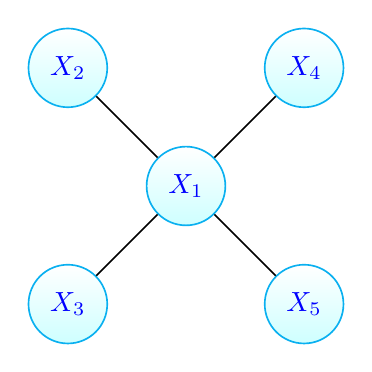
\begin{tikzpicture}[-latex, auto, node distance=4 cm and 5cm, on grid,
semithick, state/.style={circle, top color=white, bottom color=processblue!20,
draw, processblue, text=blue, minimum width=1 cm}]
  % 1 center node
  \node[state] (X1) at (3,3)        {$X_1$};
  % 4 outside nodes
  \node[state] (X2) at (4.5,1.5)    {$X_5$};
  \node[state] (X3) at (4.5,4.5)    {$X_4$};
  \node[state] (X4) at (1.5,1.5)    {$X_3$};
  \node[state] (X5) at (1.5,4.5)    {$X_2$};

\foreach \from/\to in {X1/X2,X1/X3,X1/X4,X1/X5}
    \draw[-] (\from) -- (\to);
\end{tikzpicture}
\caption{Undirected graphical model with edges between $X_i$ and $X_j$
precisely when $X_i \not\ind X_j | Z$, for $Z = (X_s : s \notin\{j,k\})$.}
\label{fig:graph_model}
\end{figure}

\item
\begin{enumerate}
\item $X_2 \ind X_3 | X_1$, since all paths from $X_2$ to $X_3$ pass through
$X_1$.
\item $X_3 \not\ind X_4$, since both are correlated with $X_1$.
\item $X_1 \not\ind X_3 | X_2$ by part (b) of problem 3, since
$\Sigma\inv_{1,3} = 1 \neq 0$.
\item $X_1 \not\ind X_5$, since $X_1$ and $X_5$ are adjacent.
\end{enumerate}

\item The graph obeys the local Markov properties in the set
\[\{X_i \ind X_j | X_1 : i,j \in \{2,\dots,5\}, i < j\}.\]

\item Note that $(X_1,X_2) \sim \mathcal{N}(0,\Sigma')$, where
\[\Sigma' = \frac{1}{15}
    \begin{bmatrix}
        9 & -3 \\
        -3 & 6
    \end{bmatrix}.\]
Thus, by part (a) of problem 3,
\fbox{$X_2 | X_1 = -3 \sim \mathcal{N}(\mu_{2|1},\Sigma_{2|1})$,} where
\[\mu_{2|1}
    = 0 + \left( -\frac{1}{5} \right)(2)(-3)
    = \mbox{\fbox{$\displaystyle \frac{6}{5}$}}\]
and
\[\Sigma_{2|1}
    = \frac{9}{15} - \left(-\frac{3}{15}\right)(3)\left(-\frac{3}{15}\right)
    = \mbox{\fbox{$\displaystyle \frac{12}{25}$.}}\]
\end{enumerate}

\item
\begin{enumerate}
\item I didn't have time to finish this problem.

\item I didn't have time to finish this problem.

\end{enumerate}

\item For $i \in \{1,\dots,n\}$, define
$Z_i := \frac{1}{h^d} K\left( \frac{\|x - X_i\|_2}{h} \right)$, so that
$\hat p_h(x) = \ol Z := \frac{1}{n} \sum_{i = 1}^n Z_i$. Note that
each $|Z_i| \leq \frac{1}{h^d} \|K\|_\infty$. We also showed previously that
$\Var[Z_i] = n \Var[\hat p_h(x)] \leq \frac{c}{h^d}$, for some $c > 0$. Thus,
applying Bernstein's Inequality,
\[\pr\left[ |\hat p_h(x) - p_h(x)| > \e \right]
    \leq 2 \exp\left( -\frac{n\e^2}{2ch^{-d}
                                        + 2\|K\|_\infty \e h^{-d}/3} \right)
    \leq c_1 e^{-n c_2 h^d \e^2},\]
for $\e \leq \e_0$, $c_1 = 2$, $c_2 = \frac{1}{2c + 2\|K\|_\infty\e_0/3}$. \qed

\newpage
\item
\begin{enumerate}
\item Let $N := N_{[]}(2\e,\Fc,L_q(P))$, and let
$\B = \{(\ell_1,u_1),\dots,(\ell_N,u_N)\}$ be a $2\e$-bracketing of $\Fc$ with
$|\B| = N$. For each $i \in \{1,\dots,N\}$, define
$f_i : [0,1] \to \R$ by
\[f_i(x) := \frac{\ell_i(x) + u_i(x)}{2}.\]
Since $\B$ is a bracketing of $\Fc$, for all $f \in \Fc$, for some
$i_f \in \{1,\dots,N\}$, $\ell_{i_f}$ and $u_{i_f}$ bracket
$f$ on $[0,1]$. Then, $\forall x \in [0,1]$,
$|f(x) - f_{i_f}(x)| \leq \frac{1}{2} |u_{i_f}(x) - \ell_{i_f}(x)|$, and so
\[\|f - f_{i_f}\|_{L_q(P)}
    \leq \frac{1}{2} \|u_{i_f} - \ell_{i_f}\|_{L_q(P)}
    \leq \e.\]
Therefore, $\C := \{f_1,\dots,f_N\}$ is an $\e$-cover of $\Fc$ with $|\C| = N$,
and so \[N(\e,\Fc,L_q(P)) \leq N_{[]}(2\e,\Fc,L_q(P)). \qed\]

\item Note that we need some additional assumptions on the functions
$\ell_1,\dots,\ell_N$ and $u_1,\dots,_N$ (since, for example, if
$X \sim$Unif$[0,1]$ and $f(x) = 1/x$, then $P f = \infty$). For simplicity
$\Fc$ is uniformly bounded (i.e., $\|f\|_\infty \leq B, \forall f \in \Fc$).

Let $N := N_{[]}(\delta/2,\Fc,L_1(P))$
$\B = \{(\ell_1,u_1),\dots,(\ell_N,u_N)\}$ be a $\delta/2$-bracketing of $\Fc$
with $|\B| = N$. Note that, for each $i \in \{1,\dots,N\}$,
\begin{equation}
|P u_i - P \ell_i|
    \leq P|u_i - \ell_i|
    = \|u_i - \ell_i\|_{L_1(P)}
    \leq \delta/2.
\label{ineq:P_L_1}
\end{equation}
Also, let
\[\e_n = \argmax_{i \in \{1,\dots,N\}, f \in \{\ell_i,u_i\}}
    |P_n f - P f|.\]
Suppose $f \in \F$. Since $\B$ is a bracketing of $\Fc$, for some
$i_f \in \{1,\dots,N\}$, $\ell_{i_f}$ and $u_{i_f}$ bracket $f$ on
$[0,1]$. If $P_n f > P f$, then, applying the triangle inequality followed by
(\ref{ineq:P_L_1}),
\begin{align*}
|P_n f - P f|
    \leq |P_n u_{i_f} - P \ell_{i_f}|
    \leq |P_n u_{i_f} - P u_{i_f}| + |P u_{i_f} - P \ell_{i_f}|
                                        + |P \ell_{i_f} - P \ell_{i_f}|
    \leq 2\e_n + \frac{\delta}{2}.
\end{align*}
Similarly, $P_n f < P f$, then
\begin{align*}
|P_n f - P f|
    \leq |P_n \ell_{i_f} - P u_{i_f}|
    \leq |P_n \ell_{i_f} - P \ell_{i_f}| + |P \ell_{i_f} - P u_{i_f}|
                                        + |P u_{i_f} - P u_{i_f}|
    \leq 2\e_n + \frac{\delta}{2}.
\end{align*}
\end{enumerate}
Applying these bounds, followed by a union bound and Hoeffding's inequality,
gives
\begin{align*}
\pr\left[ \sup_{f \in \Fc} |P_n f - P f| > \delta \right]
 &  \leq \pr\left[ 2\e_n + \delta/2 > \delta \right]    \\
 &  \leq \sum_{i \in \{1,\dots,N\},f \in \{\ell_i,u_i\}}
        \pr\left[ |P_n f - P f| > \delta/4 \right]    \\
 &  \leq \sum_{i \in \{1,\dots,N\},f \in \{\ell_i,u_i\}}
        2e^{-2n(\delta/4)^2/(2B)^2}   \\
 &  = 4N_{[]}(\delta/2,\Fc,L_1(P)) e^{-n\delta^2/(32B^2)}.   \\
\end{align*}
The desired result follows from taking $n \to \infty$. \qed
\end{enumerate}
\end{document}
